

\chapter{Materiales y Metodos:}

%Para este proyecto la principal herramienta tecnológica sera Python y en partículas se utilizaran las librerías TensorFlow, Pytorch y Ultralytics para la implementación de modelos de visión por computador , el esquema de entrenamiento y la evaluación he implementación de la herramienta. los entrenamientos y evaluaciones se realizaron en un computador personal y por medio de la plataforma google colab



\section{Datos}

Para este trabajo se utilizaron dos conjuntos de datos compuestos por imágenes digitales de láminas de herbario. Las imágenes contienen especímenes botánicos preservados junto con diversos artefactos de soporte empleados durante los procesos de catalogación, identificación y conservación, tales como etiquetas, sellos institucionales, escalas métricas y referencias de color, entre otros. La presencia y disposición de estos elementos varía entre instituciones, lo que proporciona un escenario adecuado para evaluar los modelos de visión por computador considerados en este trabajo.

El primer conjunto de datos corresponde a una muestra del Herbario Nacional Colombiano de la Universidad Nacional de Colombia~\footnote{\url{http://www.biovirtual.unal.edu.co/es/}}. Este conjunto está conformado por 987 imágenes digitales almacenadas en formato JPEG, cada una con una resolución de $500 \times 720$ píxeles. Las imágenes fueron obtenidas como parte de los procesos institucionales de digitalización y conservación del herbario. El conjunto de datos se encuentra disponible en~\footnote{\url{http://www.biovirtual.unal.edu.co/es/colecciones/search/plants/}}.

El segundo conjunto de datos corresponde al Herbario de la Universidad de Melbourne, cuya colección digital es de acceso abierto~\footnote{\url{https://www.botanic gardens.org.au/}}. Este conjunto contiene 3240 imágenes digitales almacenadas en formato JPEG con una resolución de 820 × 1200 píxeles. Al igual que en el caso anterior, las imágenes corresponden a especímenes botánicos digitalizados junto con los elementos de soporte utilizados en su documentación y preservación. El conjunto de datos puede consultarse en~\footnote{\url{https://biosciences.unimelb.edu.au/engage/herbarium/collections}}.

La utilización de dos colecciones provenientes de instituciones diferentes permite incorporar variabilidad asociada a los protocolos de preparación, digitalización y organización de los registros, proporcionando un escenario más realista para la evaluación de modelos de detección automática de artefactos en imágenes de herbario. Las principales características de los conjuntos de datos utilizados en este estudio se resumen en la Tabla~\ref{tab:datasets}. 

\begin{table}[ht]
\centering

\label{tab:datasets}
\begin{tabular}{lcc}
\hline
\textbf{Característica} & \textbf{Herbario UNAL} & \textbf{Herbario Melbourne} \\
\hline
Institución & Universidad Nacional de Colombia & Universidad de Melbourne \\
Número de imágenes & 987 & 3240 \\
Proporción del total (\%) & 23.3 & 76.7 \\
Formato de imagen & JPEG & JPEG \\
Resolución & $500 \times 720$ & $820 \times 1200$ \\
Origen de las anotaciones & Manual & Colección digital \\
Número de categorías & 15 & 18 \\
Formato de anotación final & COCO & COCO (armonizado) \\
Disponibilidad & Institucional & Acceso abierto \\
\hline
Total imágenes & \multicolumn{2}{c}{4227} \\
\hline
\end{tabular}
\caption{Resumen de los conjuntos de datos utilizados en este estudio.}
\end{table}


\subsection*{Protocolo de Anotación}

El desarrollo de métodos de visión por computador para apoyar tareas de curaduria en colecciones biológicas requiere conjuntos de datos anotados que permitan entrenar y evaluar objetivamente los algoritmos de clasificación. Aunque en los últimos años diversos trabajos han abordado el análisis automático de especímenes de herbario digitalizados, la mayoría se ha concentrado en tareas de clasificación taxonómica, reconocimiento de especies o segmentación de estructuras vegetales, existiendo relativamente pocos conjuntos de datos para la identificación de artefactos curatoriales presentes en las láminas de herbario ~\citep{guo2025review}. Debido a ello, fue necesario construir y armonizar un conjunto de anotaciones específicamente diseñado para identificar artefactos curatoriales y otros elementos de soporte utilizados en los procesos de catalogación, preservación y curaduría de colecciones botánicas.

Para la anotación de las imágenes se siguió el estándar COCO (\textit{Common Objects in Context})~\cite{COCOdataset}, uno de los formatos más utilizados en tareas de detección de objetos debido a su compatibilidad con las principales herramientas de trabajo en aprendizaje profundo y a su capacidad para representar múltiples categorías de objetos dentro de una misma imagen.

El objetivo del proceso de anotación fue identificar los principales artefactos de soporte presentes en las láminas de herbario. En este trabajo, los artefactos de soporte se definieron como todos aquellos elementos incorporados durante los procesos de preparación, catalogación y curaduría de los especímenes~\cite{}. Estos artefactos proveen información fundamental para la gestión de colecciones biológicas y representan los objetos de interés para las tareas de detección automática consideradas en este trabajo.

La definición de las categorías de anotación se realizó en conjunto con personal especializado del Herbario Nacional de Colombia, con el fin de garantizar que los elementos seleccionados correspondieran a componentes relevantes dentro de los procesos curatoriales habituales. Las categorías de anotación incluyeron elementos de identificación, documentación y referencia visual presentes en las láminas digitalizadas. Estas categorías fueron agrupadas conceptualmente en estructuras de soporte y artefactos curatoriales. Las categorías consideradas en los conjuntos de datos UNAL se presentan en la Tabla~\ref{tab:category_mapping_img}.

Las anotaciones fueron realizadas mediante cuadros delimitadores rectangulares (\textit{bounding boxes}), definidos de manera que cubrieran completamente el objeto de interés minimizando la inclusión de regiones externas. Cuando múltiples instancias de una misma categoría estaban presentes en una imagen, cada una fue anotada individualmente.

\begin{table}[ht!]
\centering

\label{tab:category_mapping_img}
\renewcommand{\arraystretch}{1.4}
\begin{tabular}{>{\centering\arraybackslash}p{3.0cm}
                >{\centering\arraybackslash}p{2.6cm}
                ||
                >{\centering\arraybackslash}p{9.2cm}}
 
% ---- Encabezado ----
\toprule
\multirow{2}{*}{\textbf{Grupo conceptual}}
  & \multicolumn{1}{c|}{\textbf{UNAL}}
  & \textbf{Melbourne} \\
  & \multicolumn{1}{c|}{\scriptsize Herbario Nacional Colombiano}
  & {\scriptsize University of Melbourne Herbarium} \\
\midrule\midrule
 
% --- Grupo 1: Códigos e identificadores digitales ------------
Códigos e\\identificadores
  & \artefacto{00Figuras/artefactos/unal/codigos.jpg}{\texttt{Mascara\_Codigos}}
  & \artefacto{00Figuras/artefactos/melbourne/small_database_label.jpg}{\texttt{small database label}}
    \artefacto{00Figuras/artefactos/melbourne/full_database_label.jpg}{\texttt{full database label}}
    \artefacto{00Figuras/artefactos/melbourne/database_label.jpg}{\texttt{database label}}
    \artefacto{00Figuras/artefactos/melbourne/number.jpg}{\texttt{number}} \\
\midrule
 
% --- Grupo 2: Referencia de color ----------------------------
Referencia de color
  & \artefacto{00Figuras/artefactos/unal/colorchecker.jpg}{\texttt{Mascara\_ColorChecker}}
  & \artefacto{00Figuras/artefactos/melbourne/swatch.jpg}{\texttt{swatch}} \\
\midrule
 
% --- Grupo 3: Descripciones y anotaciones --------------------
Descripciones\\y anotaciones
  & \artefacto{00Figuras/artefactos/unal/descripciones.jpg}{\texttt{Mascara\_Descripciones}}
  & \artefacto{00Figuras/artefactos/melbourne/handwritten_data.jpg}{\texttt{handwritten data}}
    \artefacto{00Figuras/artefactos/melbourne/annotation_label.jpg}{\texttt{annotation label}} \\
\midrule
 
% --- Grupo 4: Encabezados institucionales --------------------
Encabezados\\institucionales
  & \artefacto{00Figuras/artefactos/unal/encabezados.jpg}{\texttt{Mascara\_Encabezados}}
  & \artefacto{00Figuras/artefactos/melbourne/institutional_label.jpg}{\texttt{institutional label}}
    \artefacto{00Figuras/artefactos/melbourne/swing_tag.jpg}{\texttt{swing tag}} \\
\midrule
 
% --- Grupo 5: Escala métrica ---------------------------------
Escala métrica
  & \artefacto{00Figuras/artefactos/unal/escalas.jpg}{\texttt{Mascara\_Escalas}}
  & \artefacto{00Figuras/artefactos/melbourne/scale.jpg}{\texttt{scale}} \\
\midrule
 
% --- Grupo 6: Sellos -----------------------------------------
Sellos
  & \artefacto{00Figuras/artefactos/unal/sellos.jpg}{\texttt{Mascara\_Sellos}}
  & \artefacto{00Figuras/artefactos/melbourne/stamp.jpg}{\texttt{stamp}} \\
 
\bottomrule
\end{tabular}
\caption{Correspondencia conceptual entre las categorías de artefactos presentes
         en los conjuntos de datos UNAL y Melbourne, ilustrada con imágenes
         representativas de cada categoría. La línea vertical doble marca la
         distinción entre ambas instituciones.}
\end{table}
 

El proceso de anotación fue desarrollado por un estudiante de pregrado previamente capacitado en el protocolo establecido para este proyecto y supervisado por personal especializado del Herbario Nacional Colombiano. Con el fin de garantizar consistencia entre imágenes, se definieron criterios específicos relacionados con la delimitación de objetos parcialmente visibles, objetos superpuestos y elementos ubicados en los bordes de la imagen~\cite{}.

Con el fin de asegurar la calidad, se realizó una revisión aleatoria de un subconjunto de imágenes seleccionadas. Durante este proceso se verificó la correcta asignación de categorías, la precisión espacial de los cuadros delimitadores y el cumplimiento de los criterios de anotación definidos previamente. Las discrepancias identificadas fueron corregidas y utilizadas para refinar las directrices de anotación. Las revisiones se realizaron de manera iterativa durante el proceso de anotación.

El conjunto de datos final estuvo compuesto por dos fuentes complementarias de anotaciones. El conjunto UNAL fue anotado específicamente para este trabajo y comprende 987 imágenes y 7 categorías de objetos. Por otra parte, el conjunto Melbourne aprovechó anotaciones previamente disponibles en la colección digital de acceso abierto de la institución. Esta combinación permitió disponer simultáneamente de un conjunto de datos construido bajo criterios curatoriales locales y de un conjunto independiente generado externamente, proporcionando un escenario adecuado para evaluar la generalización de los modelos y la posterior implementación de estrategias de aprendizaje federado.

\subsection*{Integración y Armonización de las Anotaciones del Herbario de Melbourne}

A diferencia del conjunto de datos del Herbario Nacional Colombiano, cuyas anotaciones fueron generadas específicamente para este proyecto, la colección digital de la Universidad de Melbourne ya disponía de anotaciones asociadas a los especímenes como parte de la metadata pública de la colección \cite{SetMelu}. Con el fin de garantizar la compatibilidad entre ambos conjuntos de datos, se realizó un proceso de armonización y normalización de las anotaciones existentes.

Las anotaciones originales estaban almacenadas en formato JSON utilizando una representación geométrica diferente a la empleada en el conjunto UNAL. Por esta razón, se desarrolló un procedimiento automatizado para convertir todas las anotaciones al estándar COCO, transformando las coordenadas originales al formato de cuadros delimitadores (\textit{bounding boxes}) utilizado en este trabajo.

Posteriormente, se implementó un proceso de validación automática para verificar la consistencia geométrica de las anotaciones, asegurando que todos los cuadros delimitadores permanecieran contenidos dentro de los límites de la imagen. Las anotaciones inconsistentes fueron corregidas automáticamente durante el proceso de validación.

Finalmente, las categorías presentes en la colección de Melbourne fueron alineadas con las categorías definidas para el conjunto UNAL con el propósito de obtener una representación homogénea entre ambos repositorios. La Tabla~\ref{tab:category_mapping} presenta la correspondencia conceptual establecida entre las categorías de ambas colecciones y los grupos funcionales utilizados durante el proceso de armonización. Este procedimiento permitió disponer de dos conjuntos de datos compatibles entre sí, preservando la información original de cada colección y facilitando tanto la comparación directa de resultados como la implementación posterior de los experimentos de aprendizaje federado.


% \subsection*{Protocolo de Anotación - Herbario UNAL}

% El proceso de anotación de las imágenes de especímenes de herbario en este estudio siguió 
% el protocolo de anotación COCO (\textit{Common Objects in Context}), un estándar ampliamente 
% adoptado en visión por computadora que permite el etiquetado preciso y estructurado de 
% objetos dentro de imágenes mediante máscaras de segmentación basadas en polígonos, cuadros 
% delimitadores y metadatos asociados. Este formato fue seleccionado por su flexibilidad para 
% capturar la complejidad morfológica de los especímenes de herbario y su compatibilidad con 
% los marcos modernos de aprendizaje profundo. Bajo este protocolo, un equipo de estudiantes 
% de pregrado fue capacitado y encargado de anotar sistemáticamente todas las características 
% botánicas relevantes --- incluyendo hojas, tallos, flores, frutos y etiquetas --- en las 
% imágenes digitalizadas de los especímenes. El proceso de anotación abarcó especímenes de 
% dos colecciones institucionales de herbario: el Herbario Nacional y el Herbario de los 
% Jardines Botánicos Reales de Victoria (Melbourne), garantizando que el conjunto de datos 
% reflejara una muestra diversa y representativa del material botánico objeto de estudio. 
% Para garantizar la calidad y consistencia de las anotaciones, se implementó un proceso de 
% control de calidad mediante el cual se seleccionó aleatoriamente un subconjunto de 
% especímenes anotados y se revisó de forma independiente, verificando que todas las 
% etiquetas asignadas correspondieran con precisión a las características morfológicas 
% previstas y se ajustaran a las directrices de anotación establecidas.

% \begin{itemize}
%     \item \textbf{Estructuras de soporte}: etiquetas identificadoras, especímenes montados sobre cartulina y soportes de herbario.
%     \item \textbf{Artefactos}: regletas de escala, marcas de referencia y sellos de la institución.
% \end{itemize}

% La selección de estas características responde a la necesidad de obtener información relevante para la identificación automática y la extracción de metadatos estructurados. Las anotaciones fueron realizadas utilizando bounding boxes rectangulares (polígonos cuadrados), lo que permite una delimitación clara y reproducible de cada estructura de interés.

% La anotación fue realizada por un estudiante de pregrado bajo la supervisión de la directora del herbario, quien verificó la consistencia y correctitud de las etiquetas. Se consideraron un total de 15 categorías de objetos, cada una correspondiente a características morfológicas o elementos de contexto presentes en las muestras digitalizadas. Las consideraciones principales para la anotación incluyeron: (1) la exhaustividad en la detección de todas las estructuras relevantes presentes en cada muestra, (2) la consistencia en la escala de los bounding boxes independientemente de la resolución de la imagen, y (3) la precisión en el posicionamiento de los límites de caja para evitar solapes no intencionados.

% El otro set de datos trabajado fue proporcionado por la Universidad de Melbourne la cual cuenta con su colección de acceso libre \cite{SetMelu}. Se construyo una herramienta de scrapeo para descargar de manera automática todas las 3240 muestras en el mismo formato jpeg y resolución de $820 \times 1200$. Luego se procedió a proceso de etiquetado bajo el mismo formato COCO.

% \subsection*{Protocolo de Anotación - Herbario de la Universidad de Melbourne}

% Las anotaciones del herbario de Melbourne fueron originalmente proporcionadas como metadata en línea, incluyendo información descriptiva y estructural sobre cada espécimen. El proceso de normalización y estandarización se realizó en tres fases:

% \subsubsection*{Fase 1: Conversión de Formato}
% Las anotaciones originales, expresadas en formato JSON con coordenadas de centro $(x_c, y_c)$ y dimensiones $(w, h)$, fueron transformadas al estándar COCO. La transformación matemática se expresa como:

% \[
% \begin{aligned}
% x_{\text{min}} &= x_c - \frac{w}{2} \\
% y_{\text{min}} &= y_c - \frac{h}{2}
% \end{aligned}
% \]

% dondeEl resultado $(x_{\text{min}}, y_{\text{min}}, w, h)$ representa el bounding box con origen en la esquina superior izquierda, formato estándar requerido por COCO.

% \subsubsection*{Fase 2: Estandarización de Coordenadas}
% Se aplicó una función de normalización para asegurar consistencia entre las muestras de diferentes resoluciones. Para cada bounding box, se calcularon coordenadas normalizadas en el rango $[0, 1]$:

% \[
% \begin{aligned}
% x_{\text{norm}} &= \frac{x_{\text{min}}}{W} \\
% y_{\text{norm}} &= \frac{y_{\text{min}}}{H} \\
% w_{\text{norm}} &= \frac{w}{W} \\
% h_{\text{norm}} &= \frac{h}{H}
% \end{aligned}
% \]

% donde $W$ y $H$ son las dimensiones de la imagen (820 y 1200 píxeles respectivamente). Esta normalización permite que los modelos sean invariantes a pequeñas variaciones en resolución durante la inferencia posterior.

% \subsubsection*{Fase 3: Validación y Ajuste de Origen}
% Se verificó que todas las coordenadas tuvieran el origen localizado en la esquina inferior izquierda del bounding box, conforme al cumplimiento del formato COCO. Se realizó una verificación automática de:

% \[
% \text{Validez} = \begin{cases}
% 1 & \text{si } x_{\text{min}} \geq 0 \land y_{\text{min}} \geq 0 \land x_{\text{min}} + w \leq W \land y_{\text{min}} + h \leq H \\
% 0 & \text{en otro caso}
% \end{cases}
% \]

% Los bounding boxes que no cumplieron estas condiciones fueron corregidos automáticamente mediante truncamiento.

% El conjunto de anotaciones de Melbourne comprendió 18 categorías de objetos, abarcando estructuras morfológicas similares a las del conjunto UNAL pero con mayor variabilidad debido a la diversidad de técnicas de preservación utilizadas por la institución. Las consideraciones clave para esta normalización incluyeron: (1) la reproducibilidad por terceros mediante código automatizado, (2) la compatibilidad con frameworks estándar de visión por computadora (COCO API), y (3) la minimización de pérdida de información durante la transformación de coordenadas.



\section{Modelos :}


\subsection{Componentes Fundamentales de una CNN}



Las CNNs extraen representaciones jerárquicas de datos de entrada mediante capas especializadas que se describen con profundidad matemática. 

Las redes neuronales convolucionales (CNN, por sus siglas en inglés) constituyen una arquitectura ampliamente utilizada en el aprendizaje profundo debido a su capacidad para extraer representaciones jerárquicas de los datos de entrada. Su estructura se compone de diferentes tipos de capas, cada una de las cuales desempeña un papel específico en el proceso de transformación de la información. A continuación, se describen sus componentes principales.  

\subsubsection*{Capa Convolucional}
La convolución extrae patrones locales mediante productos punto entre filtros y fragmentos de entrada. Dado tensor de entrada $X \in \mathbb{R}^{H \times W \times C_{in}}$ (alto, ancho, canales) con $F$ filtros $W^{(f)} \in \mathbb{R}^{k \times k \times C_{in}}$, la salida es:

\[
A^{(f)}_{i,j} = \sum_{m=1}^{k} \sum_{n=1}^{k} \sum_{c=1}^{C_{in}} W^{(f)}_{m,n,c} \cdot X_{i+m \cdot s, j+n \cdot s, c} + b^{(f)}
\]

Donde $k$ es tamaño del filtro, $s$ es stride, $p$ es padding. Dimensiones de salida:

\[H' = \left\lfloor \frac{H + 2p - k}{s} \right\rfloor + 1\]

\textbf{Complejidad:} Número de MACs (multiplicación-acumulación): $H' \cdot W' \cdot k^2 \cdot C_{in} \cdot F$.

\textbf{Backpropagation:} Gradientes respecto a pesos:
\[\frac{\partial \mathcal{L}}{\partial W^{(f)}_{m,n,c}} = \sum_{i,j} X_{i+m\cdot s, j+n\cdot s, c} \cdot \frac{\partial \mathcal{L}}{\partial A^{(f)}_{i,j}}\]  

\subsubsection*{Funciones de Activación}
Las funciones de activación introducen no linealidad, permitiendo que redes profundas aprendan funciones complejas. La más común es ReLU:

\[
f(x) = \max(0, x), \quad f'(x) = \begin{cases} 1 & x > 0 \\ 0 & x \leq 0 \end{cases}
\]

Ventajas: eficiencia O(1), gradientes no saturados, esparcidad neuronal. Variantes modernas como Leaky ReLU ($f(x) = x$ si $x>0$ else $\alpha x$) evitan neuronas muertas.  

\subsubsection*{Capa de Pooling}
El pooling realiza submuestreo espacial reduciendo dimensionalidad y aumentando el campo receptivo. Max pooling en ventana $p \times p$ con stride $s$:

\[
Y_{i,j} = \max_{(m,n) \in \Omega} X_{i+m \cdot s, j+n \cdot s}
\]

Average pooling calcula el promedio. During backpropagation, max pooling asigna gradientes solo a posiciones máximas. Aumenta invariancia a traslaciones pequeñas.  

\subsubsection*{Batch Normalization}
Normaliza activaciones intermedias estabilizando entrenamiento. Para mini-batch $\mathcal{B}$:

\[
\mu_{\mathcal{B}} = \frac{1}{|\mathcal{B}|} \sum_{i \in \mathcal{B}} x_i, \quad \hat{x}_i = \frac{x_i - \mu_{\mathcal{B}}}{\sqrt{\sigma_{\mathcal{B}}^2 + \epsilon}}, \quad y_i = \gamma \hat{x}_i + \beta
\]

donde $\gamma, \beta$ son parámetros aprendibles. BN permite tasas de aprendizaje 35x más altas y actúa como regularizador.  

\subsubsection*{Capas Completamente Conectadas}
Combina características en vector denso: $y = Wz + b$ con complejidad O($kd$). Dropout durante entrenamiento mitiga sobreajuste:

\[
y_{\text{dropout}} = \frac{1}{1-p} (y \odot m), \quad m_i \sim \text{Bernoulli}(1-p)
\]

Factor $\frac{1}{1-p}$ (inverted dropout) asegura escala consistente durante inferencia.  

\subsubsection*{Capa de Salida y Softmax}
En clasificación multiclase, softmax transforma logits en probabilidades sobre $C$ clases:

\[
\hat{y}_i = \frac{e^{z_i}}{\sum_{j=1}^C e^{z_j}}, \quad \sum_{i=1}^C \hat{y}_i = 1
\]

Combinado con cross-entropy loss: $\mathcal{L}_{CE} = -\sum_i y_i \log(\hat{y}_i)$. El gradiente es simple: $\frac{\partial \mathcal{L}}{\partial z_i} = \hat{y}_i - y_i$, permitiendo backpropagation eficiente.  


\subsection{Flujo de Datos en una CNN}

El flujo general en una CNN se puede resumir como:

\begin{center}
\texttt{Input} $\rightarrow$ \texttt{[Conv + ReLU + Pool]}$^n$ $\rightarrow$ \texttt{Flatten} $\rightarrow$ \texttt{FC Layers} $\rightarrow$ \texttt{Output}
\end{center}
%
%\section{Ejemplo de Arquitectura CNN}

%A continuación se presenta un diagrama simplificado de una CNN típica:

%\begin{figure}[H]
%\centering
%\begin{tikzpicture}[node distance=1cm and 0.5cm, every node/.style={scale=0.8}]
%\tikzset{layer/.style={rectangle, draw, minimum width=2.5cm, minimum height=1cm}}

% Primera fila
%\node[layer] (input) {Imagen de entrada};
%\node[layer, right=of input] (conv1) {Conv + ReLU};
%\node[layer, right=of conv1] (pool1) {Max Pool};
%\node[layer, right=of pool1] (conv2) {Conv + ReLU};

% Segunda fila
%\node[layer, below=of conv1] (pool2) {Max Pool};
%\node[layer, right=of pool2] (flatten) {Flatten};
%\node[layer, right=of flatten] (fc1) {FC + ReLU};
%\node[layer, right=of fc1] (fc2) {FC + Softmax};
%\node[right=of fc2] (output) {Clasificación};

% Flechas primera fila
%\draw[->] (input) -- (conv1);
%\draw[->] (conv1) -- (pool1);
%\draw[->] (pool1) -- (conv2);

% Flechas hacia segunda fila
%\draw[->] (conv2.south) |- (pool2.north);

% Flechas segunda fila
%\draw[->] (pool2) -- (flatten);
%\draw[->] (flatten) -- (fc1);
%\draw[->] (fc1) -- (fc2);
%\draw[->] (fc2) -- (output);

%\end{tikzpicture}
%\caption{Diagrama de flujo de una CNN básica ajustado al ancho de la hoja}
%\end{figure}

\subsection{Arquitecturas Populares}

En esta sección se presenta una revisión cronológica de las arquitecturas más influyentes en la evolución de las redes convolucionales. Cada una de ellas representó un avance significativo en el campo del aprendizaje profundo y contribuyó al desarrollo de modelos más eficientes y precisos. Finalmente, se hace énfasis en las arquitecturas modernas de detección de objetos, dado que serán empleadas en el presente trabajo para la extracción y análisis de características en las muestras.  

\subsubsection{LeNet-5}  
Propuesta por LeCun et al., LeNet-5 constituye una de las primeras implementaciones exitosas de redes convolucionales, aplicada al reconocimiento de dígitos manuscritos en la base de datos MNIST. Su arquitectura se caracteriza por la combinación secuencial de capas convolucionales, funciones de activación y operaciones de \textit{pooling}, seguida de capas totalmente conectadas.  

\begin{itemize}
    \item Entrada: $32 \times 32$
    \item Conv(6 filtros, $5 \times 5$) $\rightarrow$ ReLU $\rightarrow$ Pool
    \item Conv(16 filtros, $5 \times 5$) $\rightarrow$ ReLU $\rightarrow$ Pool
    \item FC(120) $\rightarrow$ FC(84) $\rightarrow$ Softmax(10)
\end{itemize}

\subsubsection{AlexNet}  
Introducida por Krizhevsky et al. y ganadora del desafío ILSVRC 2012, AlexNet supuso un punto de inflexión en el aprendizaje profundo aplicado a visión por computadora. Esta arquitectura popularizó el uso de la función ReLU, técnicas de regularización como \textit{dropout} y el entrenamiento eficiente en unidades de procesamiento gráfico (GPU), lo que permitió entrenar redes más profundas y con mayor capacidad de generalización.  

\subsubsection{VGGNet}  
Propuesta por Simonyan y Zisserman, VGGNet destacó por el uso sistemático de filtros convolucionales de tamaño reducido ($3 \times 3$) y por su considerable profundidad (hasta 19 capas). Esta arquitectura demostró que la profundidad de la red es un factor clave para mejorar la capacidad de representación, a costa de un mayor requerimiento computacional.  

\subsubsection{ResNet}  
He et al. introdujeron las redes residuales (ResNet), cuyo aporte principal consiste en la incorporación de conexiones de atajo o \textit{skip connections}. Estas permiten que el flujo del gradiente se mantenga estable durante el entrenamiento de redes profundas, mitigando el problema del desvanecimiento del gradiente. El bloque residual se formaliza como:  

\[
\mathbf{y} = \mathcal{F}(\mathbf{x}, \{W_i\}) + \mathbf{x},
\]  

donde \(\mathcal{F}(\cdot)\) representa la transformación aprendida por las capas intermedias y \(\mathbf{x}\) la entrada original al bloque.  

\subsubsection{YOLO (You Only Look Once)}  
YOLO, propuesto por Redmon et al., reformuló la detección de objetos como un problema de regresión directa desde píxeles a coordenadas y categorías, eliminando el esquema de múltiples etapas característico de modelos como R-CNN. Esta aproximación permitió alcanzar detección en tiempo real sin sacrificar precisión.  

\begin{itemize}
    \item La imagen de entrada se divide en una grilla de $S \times S$ celdas.
    \item Cada celda predice $B$ \emph{bounding boxes} y la probabilidad de pertenencia a cada clase.
    \item La salida final posee dimensiones $S \times S \times (B \cdot 5 + C)$, donde:
    \[
    5 = (x, y, w, h, \text{confianza}), \quad C = \text{número de clases}.
    \]
\end{itemize}

Versiones más recientes, como YOLOv3 y YOLOv5, incorporan arquitecturas \textit{backbone} profundas (Darknet, CSPDarknet) y predicciones a múltiples escalas, lo que mejora significativamente el desempeño en la detección de objetos pequeños.  


\begin{figure}[H]
\centering
\includegraphics[width=0.85\textwidth]{00Figuras/yolo_architecture_diagram.png}
\caption{Arquitectura de YOLO: salida de predicciones a partir de una única pasada de la imagen}
\end{figure}

\subsubsection{SSD (Single Shot MultiBox Detector)}  
SSD constituye otra arquitectura de detección de objetos en una sola etapa. Utiliza una red convolucional base (comúnmente VGG-16) a la que se añaden capas convolucionales adicionales para realizar predicciones de cajas delimitadoras y clases a distintas escalas.  

\begin{itemize}
    \item Las predicciones se generan desde múltiples capas, permitiendo detectar objetos de diferentes tamaños.  
    \item Cada posición de la característica predice múltiples cajas con distintas relaciones de aspecto.  
    \item Se utilizan \emph{default boxes} (anclas predefinidas) en cada celda, que luego se ajustan mediante offsets aprendidos.  
\end{itemize}

La función de pérdida de SSD combina los errores de clasificación y de regresión de las cajas delimitadoras:  

\[
\mathcal{L}(x, c, l, g) = \frac{1}{N} \left( \mathcal{L}_{\text{conf}}(x, c) + \alpha \mathcal{L}_{\text{loc}}(x, l, g) \right),
\]  

donde:  

\begin{itemize}
    \item $\mathcal{L}_{\text{loc}}$: pérdida de regresión para la caja.  
    \item $\mathcal{L}_{\text{conf}}$: pérdida de entropía cruzada para las clases.  
    \item $x$: asignaciones positivas (correspondencia entre \textit{default boxes} y el \textit{ground truth}).  
    \item $N$: número de coincidencias positivas.  
\end{itemize}

\begin{figure}[H]
\centering
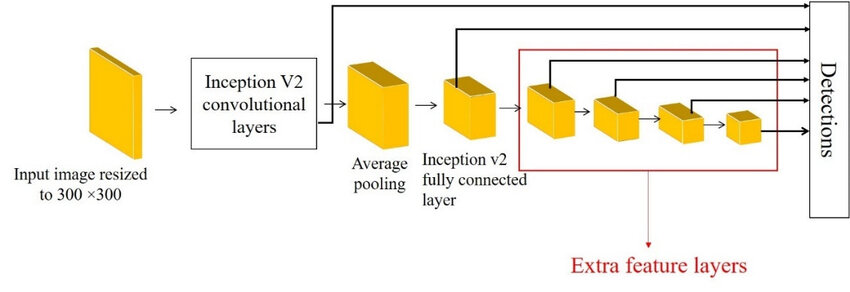
\includegraphics[width=0.85\textwidth]{00Figuras/Single-Shot-Detector-SSD-architecture.jpg}
\caption{Esquema general del detector SSD con predicciones desde múltiples escalas}
\end{figure}

\section{Métodos :}

% ------------------------------------------------------------------
\subsection{Manejo del desbalance de clases}
% ------------------------------------------------------------------

\begin{figure}[H]
    \centering
    \begin{subfigure}[b]{0.48\textwidth}
        \centering
        \includegraphics[width=\textwidth]{00Figuras/distributionLabelsUn.png}
        \caption{Distribución de etiquetas set UN}
        \label{fig:imagen1}
    \end{subfigure}
    \hfill
    \begin{subfigure}[b]{0.48\textwidth}
        \centering
        \includegraphics[width=\textwidth]{00Figuras/distribucionLabelsMelu.png}
        \caption{Distribución de etiquetas set Melbourne}
        \label{fig:imagen2}
    \end{subfigure}
    \caption{Distribución de etiquetas para los sets de datos}
    \label{fig:imagenes}
\end{figure}

Los conjuntos de datos utilizados en este trabajo presentan un marcado desbalance entre
clases: mientras que categorías como \texttt{Mascara\_Descripciones} (UNAL) o
\texttt{database label} (Melbourne) cuentan con miles de instancias etiquetadas, otras
como \texttt{small database label} están notoriamente subrepresentadas. Este desbalance
representa un desafío bien documentado en el entrenamiento de modelos de detección de
objetos~\cite{farrugiaEtAl2022}, pues los optimizadores tienden a sesgar el modelo hacia
las clases mayoritarias, degradando su capacidad de detectar las clases minoritarias.
 
Para mitigar este efecto se adoptaron dos estrategias complementarias. En primer lugar, se
aplicó \textit{data augmentation} dirigido sobre las instancias subrepresentadas, fueron
sometidas a transformaciones geométricas y fotométricas incluyendo rotaciones, cambios de
escala, variaciones de brillo y recortes aleatorios con el fin de incrementar
artificialmente la frecuencia con que estas clases aparecen durante el entrenamiento,
favoreciendo la generalización del modelo sin introducir nuevos datos reales~\cite{Goodfellow2016}.
En segundo lugar, se aprovechó el mecanismo de pesos de clase (\textit{class weights})
implementado de forma nativa en la biblioteca Ultralytics para YOLO: durante el
entrenamiento, el \textit{framework} computa automáticamente un peso inversamente
proporcional a la frecuencia de cada clase en el conjunto de entrenamiento, elevado a una
potencia controlada por el hiperparámetro \texttt{cls\_pw}~\cite{guo2025review}. Este
peso pondera la contribución de cada instancia en la función de pérdida de clasificación,
de modo que los errores cometidos sobre clases raras reciben una penalización mayor y el
modelo dedica proporcionalmente más capacidad de aprendizaje a dichas clases. Adicionalmente,
la función de pérdida focal (\textit{focal loss}) empleada por YOLO reduce la influencia
de las detecciones fáciles predominantemente las de clases mayoritarias amplificando
la señal de gradiente proveniente de los ejemplos difíciles y escasos~\cite{waltonEtAl2023}.
 
% ------------------------------------------------------------------
\subsection{Partición del conjunto de datos: entrenamiento, validación y prueba}
% ------------------------------------------------------------------
 
La partición adecuada de los datos es un paso crítico en el desarrollo de modelos de
aprendizaje profundo, pues de ella depende tanto la capacidad de generalización del modelo
como la validez estadística de las métricas reportadas~\cite{Goodfellow2016}. En este
trabajo se adoptó la proporción \textbf{70\,\%~/ 15\,\%~/ 15\,\%} para
entrenamiento, validación y prueba, respectivamente, siguiendo una práctica ampliamente
establecida en la literatura de detección de objetos~\cite{everingham2010pascal}. Esta
distribución ofrece un equilibrio entre maximizar la cantidad de datos disponibles para el
aprendizaje de los parámetros del modelo y disponer de subconjuntos de evaluación
suficientemente representativos para obtener estimaciones estables de su desempeño.
 
El subconjunto de \textbf{entrenamiento} (70\,\%) concentra la mayor parte de los datos
con el fin de que el modelo pueda aprender la variabilidad morfológica y de disposición
inherente a los artefactos de las láminas de herbario. Para el conjunto de datos UNAL esto
corresponde a 691~imágenes, y para Melbourne a 2\,268~imágenes. Dado que en promedio se
registran cinco etiquetas por lámina, el modelo fue expuesto a aproximadamente
14\,800~instancias de artefactos durante el entrenamiento. Con el propósito de garantizar
que todas las clases minoritarias estuvieran representadas en este subconjunto,
la partición se realizó de forma estratificada, asegurando la inclusión de la totalidad de
las instancias subrepresentadas antes de distribuir el remanente de forma aleatoria.
 
El subconjunto de \textbf{validación} (15\,\%) cumple una función distinta: se emplea
durante el ciclo de entrenamiento para monitorear el desempeño del modelo en datos no
vistos, detectar señales tempranas de sobreajuste y guiar la selección de
hiperparámetros  tasa de aprendizaje, tamaño del lote, número de épocas, entre otros
sin contaminar la evaluación final~\cite{Goodfellow2016}. Por su parte, el subconjunto de
\textbf{prueba} (15\,\%) permanece completamente apartado durante todo el proceso de
desarrollo y es consultado únicamente una vez, al concluir el entrenamiento, con el objeto
de obtener una estimación imparcial del desempeño del modelo ante datos completamente
nuevos~\cite{everingham2010pascal}.
 
% ------------------------------------------------------------------
\subsection{Selección y justificación de las métricas de evaluación}
% ------------------------------------------------------------------
 
La evaluación de modelos de detección de objetos requiere métricas capaces de capturar
simultáneamente la calidad de la clasificación y la precisión de la localización espacial
de los objetos detectados. En este trabajo se seleccionaron tres métricas complementarias:
\textbf{Precisión} (\textit{Precision}), \textbf{puntuación F1} (\textit{F1 score}) e
\textbf{Intersección sobre Unión} (\textit{Intersection over Union}, IoU).
 
La \textit{Precisión} se define como la fracción de detecciones positivas que son
efectivamente correctas:
 
\begin{equation}
  \text{Precisión} = \frac{VP}{VP + FP},
  \label{eq:precision}
\end{equation}
 
\noindent donde $VP$ denota los verdaderos positivos y $FP$ los falsos positivos.
Esta métrica cuantifica la confiabilidad de las detecciones del modelo: un valor alto
indica que la mayoría de los artefactos señalados por el detector corresponden
efectivamente a artefactos reales, minimizando falsas alarmas. En el contexto de la
curaduría de herbarios, una alta precisión es especialmente relevante cuando el objetivo
es verificar la completitud de los artefactos, pues las detecciones espurias podrían
introducir ruido en los reportes automáticos de calidad~\cite{powers2020evaluation}.
 
La \textit{puntuación F1} constituye la media armónica entre la precisión y la
exhaustividad (\textit{recall}):
 
\begin{equation}
  F1 = \frac{2 \cdot \text{Precisión} \cdot \text{Recall}}
            {\text{Precisión} + \text{Recall}},
  \label{eq:f1}
\end{equation}
 
\noindent donde el \textit{recall} mide la fracción de artefactos reales que el modelo
logra detectar ($VP / (VP + FN)$). La puntuación F1 es la métrica más apropiada para
escenarios con clases desbalanceadas~\cite{powers2020evaluation}, como los que caracterizan
a los conjuntos de datos de este trabajo, ya que penaliza por igual los errores de omisión
(artefactos no detectados) y los de comisión (detecciones incorrectas), ofreciendo una
visión integrada y equilibrada del desempeño del modelo por clase.
 
Finalmente, el \textit{IoU} cuantifica el grado de solapamiento espacial entre la caja
delimitadora predicha por el modelo ($B_p$) y la caja delimitadora de referencia ($B_{gt}$):
 
\begin{equation}
  \text{IoU} = \frac{|B_p \cap B_{gt}|}{|B_p \cup B_{gt}|},
  \label{eq:iou}
\end{equation}
 
\noindent y toma valores en el intervalo $[0, 1]$, donde 1 corresponde a un solapamiento
perfecto. Esta métrica es indispensable en tareas de detección de objetos porque evalúa
no solo si el modelo identifica correctamente la categoría del artefacto, sino también
con qué exactitud delimita su posición y extensión en la imagen~\cite{everingham2010pascal}.
Una localización precisa resulta crítica para tareas curatoriales como la ofuscación
de información sensible o la remoción de artefactos previo al análisis morfológico, donde
una caja delimitadora inexacta podría cubrir o exponer inadvertidamente regiones de interés.
En este trabajo se empleó un umbral de $\text{IoU} \geq 0.5$ para determinar si una
detección constituye un verdadero positivo, siguiendo la convención establecida por el
protocolo de evaluación PASCAL VOC~\cite{everingham2010pascal} y adoptada de forma
generalizada en trabajos de detección en imágenes de herbario~\cite{waltonEtAl2023,
hussein2021}.




% Luego se procedió con proceso de selección de la arquitectura apropiada, para esto se realizaron los respectivos entrenamientos por cada modelo y se calculo medidas de confiabilidad y precisión sobre las predicciones del modelo. Las métricas estudiadas con profundidad matemática son:

% \subsection{Recall}
% Mide la capacidad del modelo de identificar todas las instancias positivas presentes:

% \[\text{Recall} = \frac{TP}{TP + FN} = P(\text{predicción positiva} \mid \text{verdad positiva})\]

% donde $TP$ = verdaderos positivos, $FN$ = falsos negativos. Recall alto es crítico en detención de objetos para no perder especímenes.

% \subsection{Precisión}
% Mide qué proporción de predicciones positivas son realmente correctas:

% \[\text{Precisión} = \frac{TP}{TP + FP} = P(\text{verdad positiva} \mid \text{predicción positiva})\]

% donde $FP$ = falsos positivos. Precisión alta minimiza detecciones falsas.

% \subsection{F1-score}
% Media armónica de precisión y recall, proporcionando balance único:

% \[F1 = \frac{2 \cdot TP}{2 \cdot TP + FP + FN} = 2 \cdot \frac{\text{Precisión} \cdot \text{Recall}}{\text{Precisión} + \text{Recall}}\]

% La media armónica penaliza desbalances severos. Es preferred en datasets desbalanceados como el de herbario.

% \subsection{Confianza}
% Representa la probabilidad estimada por el modelo o probabilidad condicional:

% \[\text{Confianza}(c) = P(y=c \mid x) = \text{softmax}(z)_c\]

% Valores > 0.5 típicamente indican detecciones válidas en visión por computadora.

% \subsection{Mean Average Precision (mAP)}
% Métrica estándar para detención de objetos, calculada en dos fases:

% \subsubsection*{Fase 1: Intersección sobre Unión (IoU)}
% Para cada predicción, se computa IoU entre caja predicha y verdad:

% \[\text{IoU} = \frac{\text{Área de intersección}}{\text{Área de unión}} = \frac{|B_{pred} \cap B_{gt}|}{|B_{pred} \cup B_{gt}|}\]

% Predicciones con IoU > umbral (típicamente 0.5) son verdaderos positivos.

% \subsubsection*{Fase 2: Curva Precisión-Recall}
% Para cada clase, se ordena predicciones por confianza decreciente y se computa Average Precision (AP) como el área bajo la curva:

% \[AP = \int_0^1 P(r) \, dr\]

% El mAP es el promedio de AP sobre todas las clases:

% \[mAP = \frac{1}{N} \sum_{i=1}^{N} AP_i\]

%Una vez consideradas estas métricas y con el modelo que mejor se adapte a nuestras necesidades se construyo la arquitectura necesaria para un esquema federado , la cual consiste de un servidor en donde se compilan los pesos de los diferentes modelos desplegados en los clientes, en esta sección se experimento con los principales algoritmos de agregación para el modelo general los cuales son :
\section{Modelo Federado}
 
La inteligencia artificial con arquitectura federada surge como una respuesta a las
crecientes preocupaciones por la privacidad y la seguridad de los datos en el entrenamiento
de modelos de aprendizaje profundo. Su origen se remonta a las investigaciones de Google
en 2016~\citep{mcmahan2017communication}, con el desarrollo de \textit{Federated Learning},
una técnica que permite entrenar modelos directamente sobre los datos de cada participante
sin necesidad de centralizarlos. Esta arquitectura distribuye el proceso de aprendizaje
entre múltiples nodos como teléfonos inteligentes o servidores institucionales que
colaboran para construir un modelo común sin compartir información sensible. A lo largo del
tiempo, la tecnología ha evolucionado incorporando técnicas más avanzadas de agregación de
parámetros, encriptación homomórfica y aprendizaje con privacidad diferencial, lo que ha
reforzado su utilidad en entornos donde la confidencialidad de los datos es
crítica~\citep{bonawitz2016practicalsecureaggregationfederated}.
 
Actualmente, los modelos federados se aplican en sectores como la salud, la banca, las
telecomunicaciones y el internet de las cosas (IoT), donde el acceso a datos distribuidos
es vital y al mismo tiempo restringido. Hospitales, por ejemplo, pueden colaborar para
mejorar modelos de diagnóstico sin intercambiar historiales clínicos de pacientes. El
estado del arte incluye innovaciones como el \textit{federated transfer learning}, que
permite combinar conocimientos de diferentes dominios, y el uso de modelos multimodales
en entornos federados. A pesar de los avances, persisten desafíos técnicos como la
heterogeneidad de los datos, las limitaciones de cómputo en los nodos cliente y la
sincronización eficiente entre rondas. No obstante, la arquitectura federada se consolida
como una de las líneas más prometedoras para un desarrollo ético y escalable de la
inteligencia artificial.
 
% ------------------------------------------------------------------
\subsection{Aprendizaje federado en el contexto de herbarios digitales}
% ------------------------------------------------------------------
 
En el contexto particular de este trabajo, el aprendizaje federado ofrece ventajas
concretas que van más allá de los argumentos generales de privacidad. Los herbarios
digitales operan bajo restricciones institucionales que hacen inviable la centralización
de sus imágenes: los metadatos de localización de especies amenazadas son confidenciales
por razones de conservación; los derechos de imagen sobre los especímenes pertenecen a las
instituciones que los custodian; y los acuerdos de colaboración entre herbarios
frecuentemente prohíben la redistribución de los datos primarios.
 
El aprendizaje federado permite que el \textbf{Herbario Nacional Colombiano (UNAL)} y el
\textbf{University of Melbourne Herbarium} colaboren en el entrenamiento de un detector de
artefactos sin transferir una sola imagen. Adicionalmente, la arquitectura distribuida
habilita dos ventajas operativas de alto valor:
 
\begin{enumerate}
    \item \textbf{Mejora cruzada entre instituciones.} El modelo del nodo UNAL se beneficia
    de los patrones visuales aprendidos sobre los once tipos de artefactos de Melbourne
    escalas, etiquetas impresas, sellos de distintos formatos aunque no los clasifique
    por su nombre local. A la inversa, Melbourne mejora su capacidad de reconocer los
    artefactos característicos del protocolo colombiano. Este intercambio de conocimiento
    visual ocurre sin compartir datos, únicamente a través de los pesos del \textit{backbone}.
 
    \item \textbf{Escalabilidad sin re-etiquetado.} Una tercera institución por ejemplo el
    Kew Gardens o el Smithsonian puede incorporarse al sistema federado entrenando su
    propio nodo con su esquema de etiquetado local, sin necesidad de adaptar ni re-etiquetar
    sus colecciones para hacerlas compatibles con las de los demás participantes.
\end{enumerate}
 
La Figura~\ref{fig:federated_herbarium} ilustra la arquitectura federada adoptada en este
trabajo, en la que cada institución mantiene sus datos y su cabeza de clasificación de
forma local, mientras que el \textit{backbone} del detector se agrega de forma centralizada.
 
\begin{figure}[H]
    \centering
    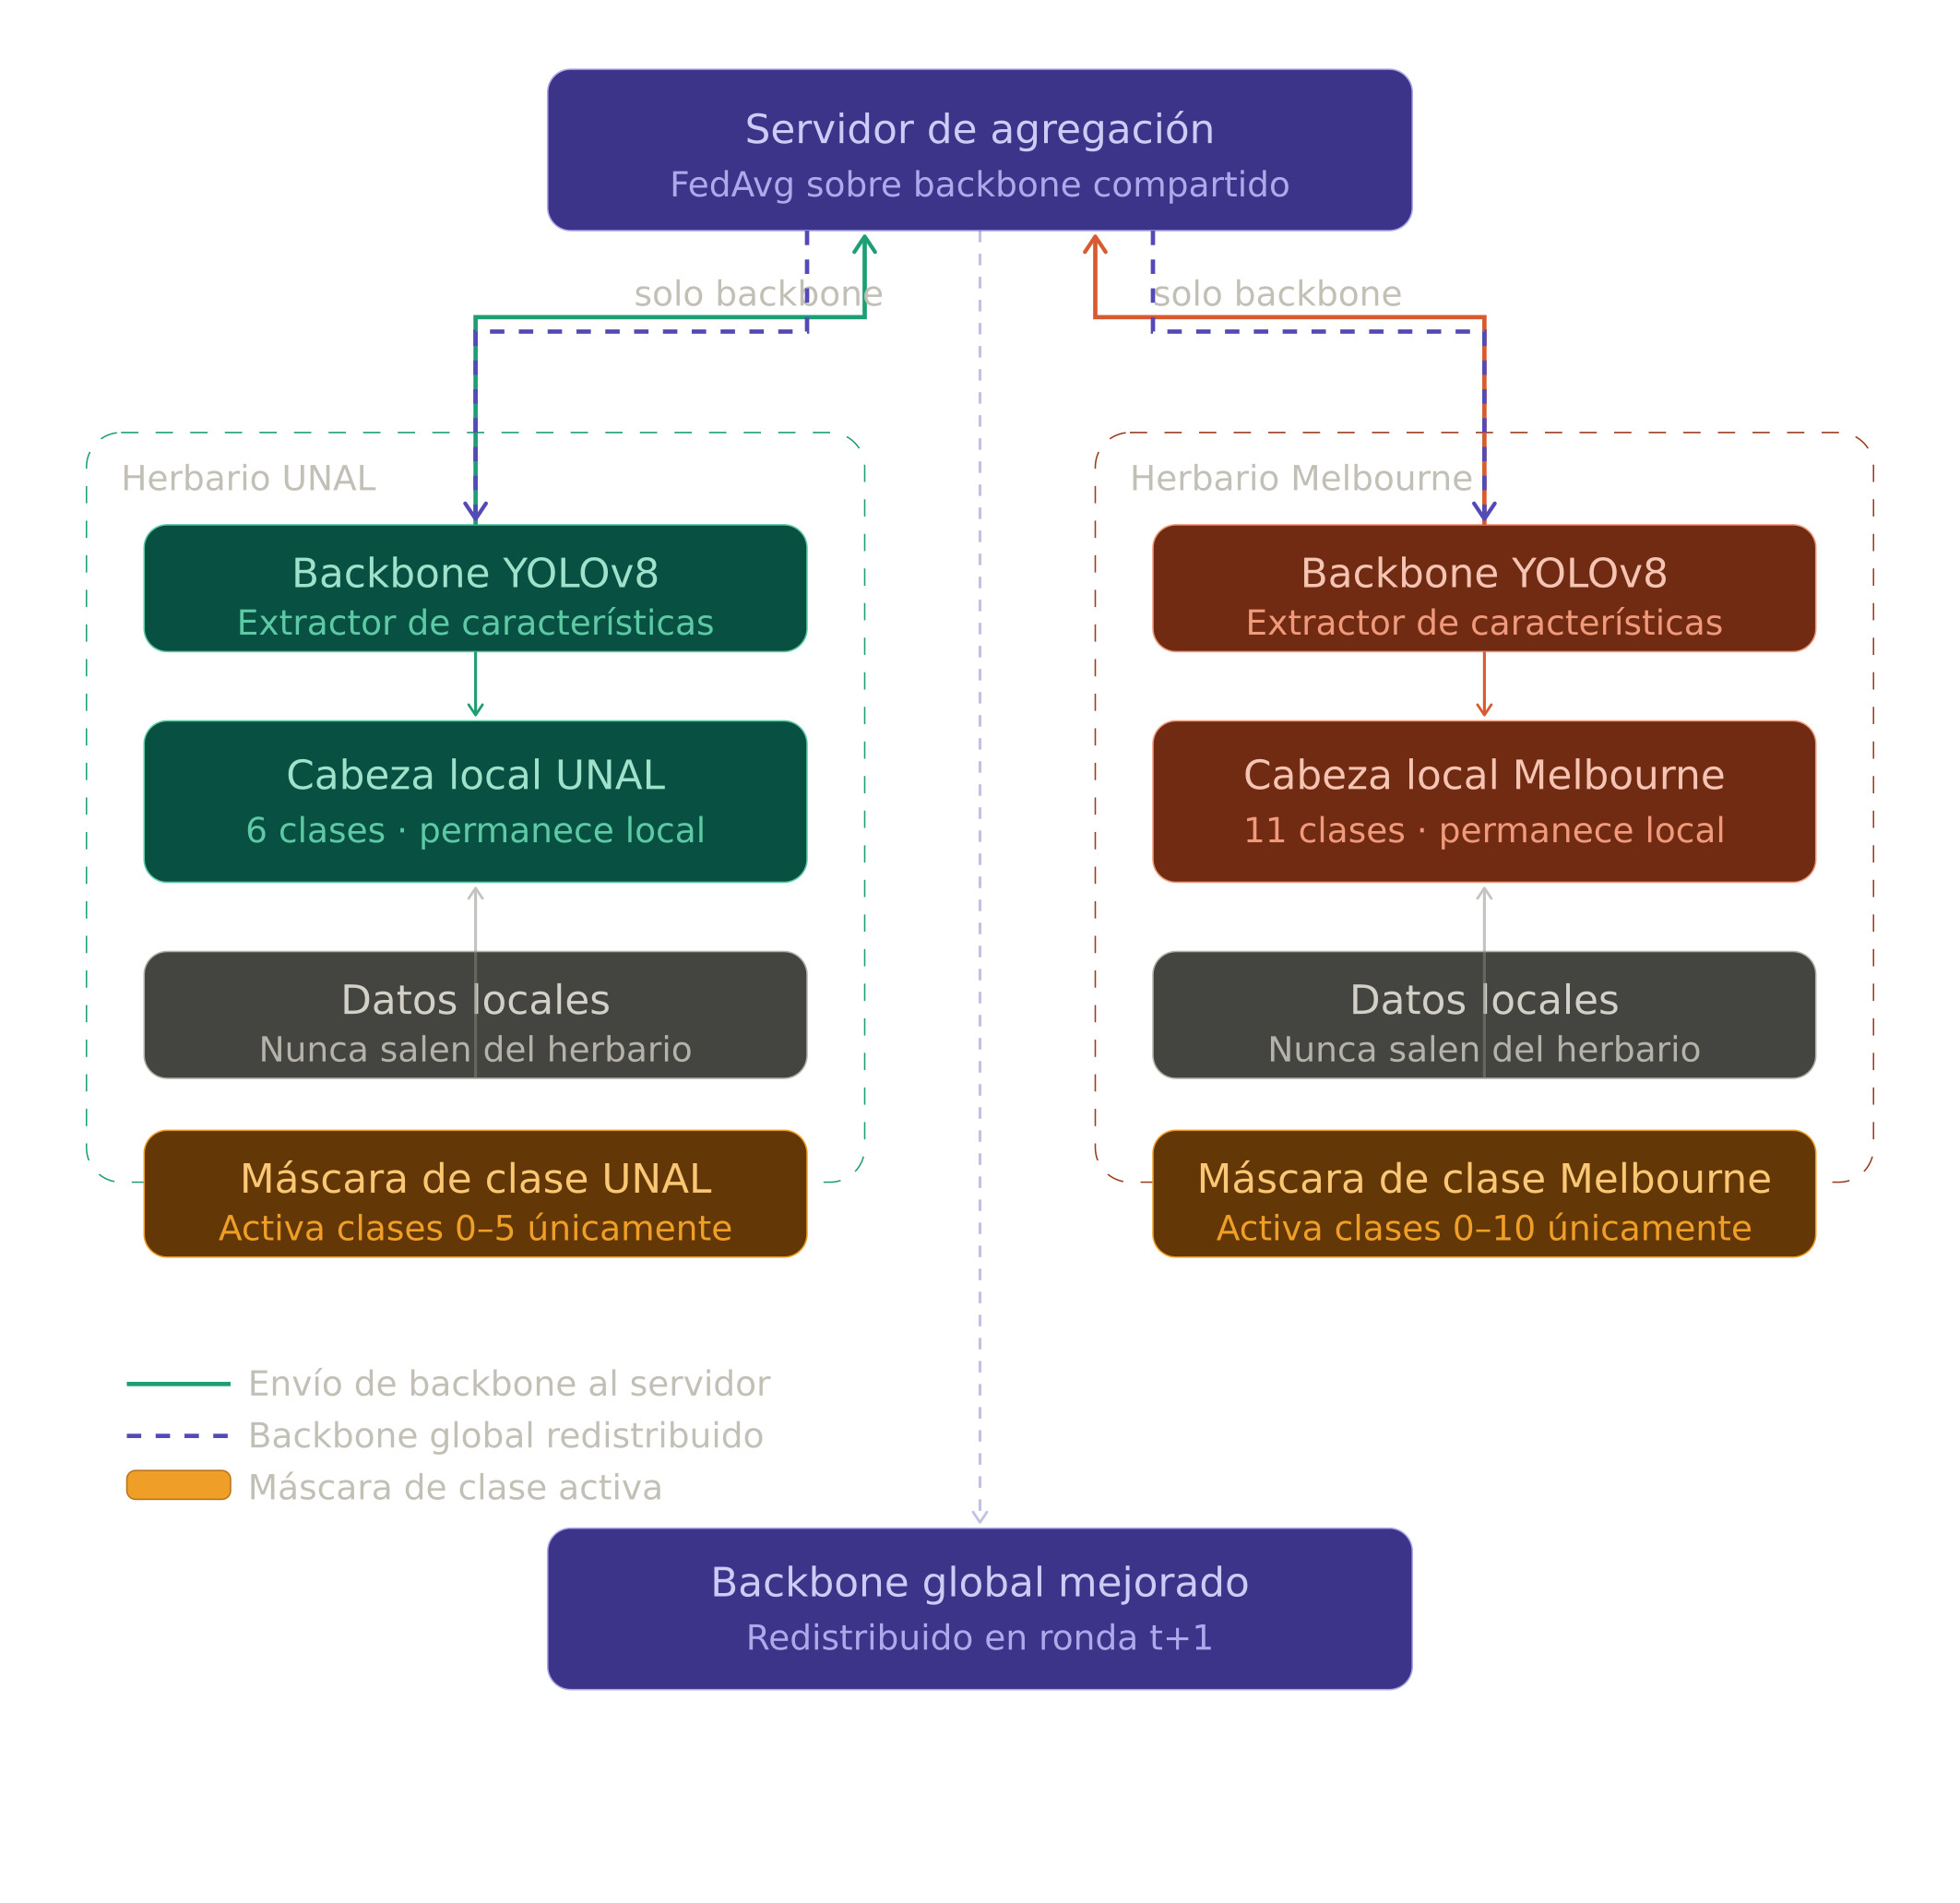
\includegraphics[width=0.92\textwidth]{00Figuras/federated_herbarium_strategy.jpg}
    \caption{Arquitectura federada para la detección de artefactos en registros digitales
             de herbario. Cada nodo institucional (UNAL: 6 clases, Melbourne: 11 clases)
             entrena localmente un modelo YOLOv8 con sus propios datos, que nunca abandonan
             la institución. Solo los pesos del \textit{backbone} el extractor de
             características compartido se envían al servidor de agregación mediante
             FedAvg. Las cabezas de clasificación locales y las máscaras de clase
             (destacadas en naranja) permanecen en cada nodo, evitando la confusión entre
             los vocabularios de etiquetado de ambas instituciones.}
    \label{fig:federated_herbarium}
\end{figure}
 
% ------------------------------------------------------------------
\subsection{Fases del entrenamiento federado}
% ------------------------------------------------------------------
 
El proceso de aprendizaje federado se estructura en fases bien definidas que permiten una
coordinación eficiente entre clientes y servidor:
 
\subsubsection*{Fase 1: Inicialización global}
 
En esta fase inicial, el servidor central genera un modelo global $w_0$ con parámetros
inicializados aleatoriamente. Este modelo es distribuido a todos los clientes
$k \in \{1, 2, \ldots, K\}$, de modo que todos reciben una réplica idéntica:
 
\[
w_0^{(k)} = w_0 \quad \forall\, k
\]
 
\subsubsection*{Fase 2: Entrenamiento local}
 
Cada cliente $k$ realiza un entrenamiento local utilizando únicamente sus datos
$D_k$. Durante $E$ épocas locales, el cliente computa el descenso de gradiente
estocástico:
 
\[
w_t^{(k,e+1)} = w_t^{(k,e)} - \eta \,\nabla F_k\!\left(w_t^{(k,e)}, B\right)
\]
 
donde $w_t^{(k,e)}$ son los parámetros del cliente $k$ en la época local $e$ de la ronda
$t$, $\eta$ es la tasa de aprendizaje local, $B \subset D_k$ es un mini-lote de datos y
$F_k(w) = \frac{1}{|D_k|} \sum_{(x,y) \in D_k} \ell(\mathrm{model}(w, x),\, y)$
es la función de pérdida local. Al completarse las $E$ épocas, el cliente obtiene el modelo
actualizado $w_t^{(k,E)}$.
 
\subsubsection*{Fase 3: Comunicación de parámetros}
 
Cada cliente transmite sus parámetros actualizados $w_t^{(k,E)}$ al servidor central.
En este trabajo se utilizó transmisión sin compresión ($\rho = 1$), aunque es posible
aplicar técnicas de cuantización para reducir el ancho de banda requerido:
 
\[
\tilde{w}_t^{(k)} = \mathrm{Comprime}\!\left(w_t^{(k,E)},\, \rho\right)
\]
 
\subsubsection*{Fase 4: Agregación global}
 
El servidor agrega los parámetros recibidos de todos los clientes mediante uno de los
algoritmos descritos en la Sección~\ref{subsec:agregacion}, produciendo un nuevo modelo
global $w_{t+1}$ que es redistribuido a todos los nodos.
 
\subsubsection*{Fase 5: Criterio de parada}
 
El proceso iterativo se repite hasta cumplirse alguna de las siguientes condiciones:
 
\[
\text{Criterio de parada} =
\begin{cases}
    \text{Continúa} & \text{si } |\mathcal{L}_t - \mathcal{L}_{t-1}| > \varepsilon
                       \;\text{ y }\; t < T_{\max} \\
    \text{Detiene}  & \text{en otro caso}
\end{cases}
\]
 
donde $\mathcal{L}_t$ es la pérdida global promediada en la ronda $t$, $\varepsilon$ es el
umbral de convergencia y $T_{\max}$ es el número máximo de rondas permitidas.
 
% ------------------------------------------------------------------
\subsection{Estrategias para la heterogeneidad de clases entre nodos}
\label{subsec:estrategias_clases}
% ------------------------------------------------------------------
 
El caso concreto de este trabajo presenta un desafío que va más allá del aprendizaje
federado estándar: los dos nodos participantes no comparten el mismo vocabulario de clases.
UNAL emplea seis categorías de artefactos y Melbourne emplea once, con correspondencias
conceptuales parciales pero sin identidad directa (véase la Tabla~\ref{tab:category_mapping_img}).
Esto impide una aplicación directa de FedAvg, que asume que todos los nodos comparten
exactamente la misma arquitectura de salida. A continuación se presentan las tres
estrategias contempladas, en orden creciente de complejidad.
 
\subsubsection{Estrategia 1: Espacio de clases unificado}
 
La aproximación más sencilla consiste en definir un vocabulario global de clases fusionando
los esquemas de ambas instituciones mediante el mapeo conceptual de la
Tabla~\ref{tab:category_mapping_img}. Las once etiquetas de Melbourne se colapsan en los seis
grupos conceptuales de UNAL, de modo que ambos nodos operan con una cabeza de clasificación
idéntica de seis salidas. La agregación FedAvg puede aplicarse sin modificaciones porque
las arquitecturas son plenamente compatibles.
 
La principal limitación de esta estrategia es la pérdida de granularidad: al colapsar
\texttt{small database label}, \texttt{full database label} y \texttt{database label} en
una única clase \textit{Códigos e identificadores}, el modelo pierde la capacidad de
distinguir entre etiquetas de base de datos de distintos tamaños, información que puede
ser relevante para tareas curatoriales específicas de Melbourne.
 
\subsubsection{Estrategia 2: \textit{Backbone} compartido con cabezas locales}
 
Una alternativa más flexible consiste en separar el modelo en dos componentes con
comportamientos distintos durante la federación:
 
\begin{itemize}
    \item \textbf{\textit{Backbone} (capas convolucionales):} aprende representaciones
    visuales generales bordes, texturas, formas independientes del esquema de etiquetado.
    Este componente \emph{sí} se comparte y se agrega mediante FedAvg.
 
    \item \textbf{Cabeza de clasificación:} mapea las representaciones visuales a las clases
    propias de cada institución. Este componente \emph{permanece local} en cada nodo y no
    participa en la agregación.
\end{itemize}
 
La actualización global se restringe entonces al \textit{backbone}:
 
\[
w_{t+1}^{\mathrm{back}} = \sum_{k \in \{\mathrm{UNAL},\,\mathrm{Melb}\}}
    \frac{n_k}{N}\, w_t^{(k,E,\mathrm{back})}
\]
 
La intuición detrás de esta estrategia es que reconocer visualmente un sello institucional
o una escala métrica comparte características de bajo nivel gradientes de color, patrones
de texto, contraste independientemente de cómo se denomine esa clase en cada institución.
El \textit{backbone} federado aprende esas características de forma conjunta; cada nodo las
especializa a través de su propia cabeza. Esta estrategia preserva la granularidad de ambos
esquemas y resulta especialmente atractiva cuando los vocabularios de clase son
substancialmente distintos.
 
\subsubsection{Estrategia 3: Espacio de \textit{embedding} compartido con máscaras de clase}
\label{subsubsec:estrategia3}
 
Esta es la estrategia adoptada en el presente trabajo. En lugar de restringir la
federación al \textit{backbone} o de colapsar los vocabularios, se define un espacio de
salida unificado con $C = C_{\mathrm{UNAL}} + C_{\mathrm{Melbourne}} = 6 + 11 = 17$
clases. El modelo completo incluyendo la cabeza de clasificación tiene arquitectura
idéntica en todos los nodos y participa íntegramente en la agregación FedAvg. La clave que
resuelve el conflicto entre vocabularios es el uso de \textbf{máscaras de clase} durante
el entrenamiento local.
 
Formalmente, para cada cliente $k$, se define una máscara binaria
$m_k \in \{0,1\}^C$ tal que:
 
\[
m_k^{(c)} =
\begin{cases}
    1 & \text{si la clase } c \text{ pertenece al vocabulario del nodo } k \\
    0 & \text{en otro caso}
\end{cases}
\]
 
Durante el cómputo de la pérdida local, el gradiente se anula para las clases
desconocidas en el nodo $k$:
 
\[
\mathcal{L}_k^{\mathrm{masked}}(w) =
    \sum_{c=1}^{C} m_k^{(c)} \cdot
    \ell_c\!\left(\mathrm{model}(w, x),\, y\right)
\]
 
De este modo, el nodo UNAL ($m_{\mathrm{UNAL}}^{(c)} = 1$ para $c \in \{0,\ldots,5\}$)
solo penaliza al modelo por los errores en sus seis clases propias, y el nodo Melbourne
($m_{\mathrm{Melb}}^{(c)} = 1$ para $c \in \{0,\ldots,10\}$) solo penaliza por sus once
clases. Las salidas correspondientes a clases desconocidas en cada nodo no reciben señal
de gradiente y no contaminan el aprendizaje.
 
En inferencia, la institución activa únicamente las salidas de su vocabulario para la
toma de decisiones, ignorando el resto. Esta estrategia presenta tres ventajas respecto a
las anteriores:
 
\begin{enumerate}
    \item \textbf{Preservación total de la granularidad.} Ningún esquema de etiquetado
    es colapsado ni simplificado; ambas instituciones mantienen intacta su taxonomía de
    artefactos.
 
    \item \textbf{Agregación global completa.} A diferencia de la Estrategia~2, la cabeza
    de clasificación también se beneficia de la federación, pues las salidas activas de un
    nodo son indirectamente informadas por las representaciones aprendidas en el otro.
 
    \item \textbf{Extensibilidad natural.} La incorporación de un tercer nodo con un
    vocabulario diferente requiere únicamente definir su máscara $m_k$ y añadir las clases
    nuevas al espacio de salida, sin modificar la arquitectura ni re-entrenar los nodos
    existentes.
\end{enumerate}
 
% ------------------------------------------------------------------
\subsection{Métodos de agregación}
\label{subsec:agregacion}
% ------------------------------------------------------------------
 
La agregación de parámetros constituye el núcleo del aprendizaje federado, permitiendo que
múltiples modelos locales se combinen en un único modelo global. A continuación se presentan
los algoritmos empleados en este trabajo.
 
\subsubsection{Federated Averaging (FedAvg)}
 
FedAvg~\citep{mcmahan2017communication} es el algoritmo fundacional del aprendizaje
federado. Opera mediante un promedio ponderado por la proporción de datos locales:
 
\begin{equation}
    w_{t+1} = \sum_{k=1}^{K} \frac{n_k}{N}\, w_t^{(k,E)}
    \label{eq:fedavg}
\end{equation}
 
donde $n_k = |D_k|$ es el número de muestras en el cliente $k$ y $N = \sum_{k} n_k$.
La ponderación por $n_k / N$ asegura que los nodos con mayor volumen de datos en este
caso Melbourne, con 3\,240 imágenes frente a las 988 de UNAL ejerzan mayor influencia
en la actualización global. Bajo supuestos de convexidad y gradientes acotados, la
convergencia de FedAvg satisface:
 
\[
\mathbb{E}\!\left[\|\nabla F(w_T)\|^2\right] \leq
    \mathcal{O}\!\left(\frac{1}{\sqrt{T}} + \frac{\sigma^2}{K\beta T}\right)
\]
 
donde $\sigma^2$ es la varianza del gradiente y $\beta$ la constante de suavidad.
 
\subsubsection{Federated Stochastic Variance Reduced Gradient (FedSVRG)}
 
FedSVRG mejora FedAvg mediante la introducción de un término corrector de varianza que
mitiga el efecto de la heterogeneidad de datos. En cada cliente $k$, la actualización
local se corrige como:
 
\begin{equation}
    g^{(k)} = \nabla F_k\!\left(w_t^{(k)}\right) -
               \nabla F_k\!\left(\bar{w}_{t-1}\right) + \bar{g}_{t-1}
\end{equation}
 
donde $\bar{g}_{t-1} = \frac{1}{K}\sum_{k} \nabla F_k(\bar{w}_{t-1})$ es el gradiente
promedio global de la ronda anterior. El término corrector
$p^{(k)} = \nabla F_k(\bar{w}_{t-1}) - \bar{g}_{t-1}$ captura la desviación de los
gradientes locales respecto al promedio global, reduciendo la varianza acumulada a:
 
\[
\mathrm{Var}\!\left[g^{(k)}\right] \leq
    \mathcal{O}\!\left(\sigma_{\mathrm{loc}}^2 + \sigma_{\mathrm{global}}^2\right)
\]
 
\subsubsection{FedProx  Federated Proximal}
 
FedProx~\citep{reddi2020adaptive} aborda la heterogeneidad mediante un término
regularizador proximal que mantiene los modelos locales cercanos al modelo global.
La función objetivo en cada cliente se modifica como:
 
\begin{equation}
    \mathcal{L}_k^{\mathrm{FedProx}}(w) =
        \frac{1}{|D_k|} \sum_{(x,y) \in D_k} \ell\!\left(\mathrm{model}(w, x),\, y\right)
        + \frac{\mu}{2}\,\|w - w_t\|_2^2
\end{equation}
 
donde $\mu$ es el coeficiente de regularización proximal. Cuando $\mu \to 0$, FedProx
recupera el comportamiento de FedAvg; a medida que $\mu$ aumenta, las actualizaciones
locales quedan más ancladas al modelo global. FedProx proporciona garantías de convergencia
bajo heterogeneidad fuerte (datos \textit{non-IID}):
 
\[
\mathbb{E}\!\left[\|\nabla F(w_T)\|^2\right] =
    \mathcal{O}\!\left(\frac{1}{T} + \frac{1}{\sqrt{T}}\right)
\]
 
\subsubsection{FedOpt  Optimización federada adaptativa}
 
FedOpt~\citep{reddi2020adaptive} generaliza los métodos de optimización adaptativa (Adam,
AdaGrad) al contexto federado. En lugar de promediar solo los parámetros, FedOpt acumula
momentos de optimización en el servidor:
 
\begin{align}
    m_{t+1} &= \beta\, m_t + (1-\beta)\,\bar{g}_t \\
    w_{t+1} &= w_t - \eta\, m_{t+1}
\end{align}
 
La variante con momentos de segundo orden (Adam federado) incorpora:
 
\begin{align}
    v_{t+1}  &= \alpha\, v_t + (1-\alpha)\,\bar{g}_t^2 \\
    w_{t+1}  &= w_t - \eta\,\frac{m_{t+1}}{\sqrt{v_{t+1}} + \varepsilon}
\end{align}
 
adaptando la tasa de aprendizaje por dimensión, lo que resulta especialmente útil
cuando los gradientes presentan alta variabilidad entre nodos.
 
\subsubsection{FedAvgM  FedAvg con \textit{momentum}}
 
FedAvgM extiende FedAvg incorporando \textit{momentum} en la agregación global, manteniendo
un promedio móvil exponencial de los cambios de parámetros entre rondas:
 
\begin{align}
    m_t      &= \beta\, m_{t-1} + (1-\beta)\left(w_t - w_{t-1}^{\mathrm{agg}}\right) \\
    w_{t+1}  &= w_t + \eta\, m_t
\end{align}
 
O, de forma equivalente:
 
\begin{equation}
    w_{t+1} = w_t + \eta\left[
        \beta\, m_{t-1} + (1-\beta) \sum_{k=1}^{K} \frac{n_k}{N}
        \left(w_t^{(k,E)} - w_t\right)
    \right]
\end{equation}
 
El \textit{momentum} añade inercia a la actualización global, acelerando la convergencia
en direcciones consistentes y atenuando las oscilaciones causadas por la variabilidad entre
rondas. La tasa de convergencia con \textit{momentum} mejora a:
 
\[
\mathbb{E}\!\left[\|\nabla F(w_T)\|\right] =
    \mathcal{O}\!\left(\frac{1}{T^{0.75}}\right)
\]
 
frente a $\mathcal{O}(1/\sqrt{T})$ de FedAvg sin \textit{momentum}.
 
Los resultados experimentales de los algoritmos presentados se discuten en la siguiente
sección.